%% LyX 2.2.3 created this file.  For more info, see http://www.lyx.org/.
%% Do not edit unless you really know what you are doing.
\documentclass[oneside,english]{amsart}
\usepackage{lmodern}
\usepackage{lmodern}
\usepackage[T1]{fontenc}
\usepackage{geometry}
\geometry{verbose,tmargin=1in,bmargin=1in,lmargin=1in,rmargin=1in}
\usepackage{babel}
\usepackage{mathtools}
\usepackage{amstext}
\usepackage{amsthm}
\usepackage{amssymb}
\usepackage{setspace}
\usepackage{graphicx}
\usepackage{caption}
\usepackage{subcaption}
\doublespacing
\usepackage[unicode=true,
 bookmarks=false,
 breaklinks=false,pdfborder={0 0 1},backref=section,colorlinks=false]
 {hyperref}

\makeatletter
%%%%%%%%%%%%%%%%%%%%%%%%%%%%%% Textclass specific LaTeX commands.
\numberwithin{equation}{section}
\numberwithin{figure}{section}
\theoremstyle{plain}
\newtheorem{thm}{\protect\theoremname}
  \theoremstyle{definition}
  \newtheorem{defn}[thm]{\protect\definitionname}

%%%%%%%%%%%%%%%%%%%%%%%%%%%%%% User specified LaTeX commands.




\usepackage{babel}
\providecommand{\theoremname}{Theorem}

\makeatother

  \providecommand{\definitionname}{Definition}
\providecommand{\theoremname}{Theorem}

\begin{document}

\title{Locally stationary process and its applications: A Brief Tutorial}

\author{Hengrui Luo and Kori Khan}
\maketitle

\section{Introduction to Locally Stationary Processes}

Nonstationary data occurred in various scenarios like spatial statistics,
geology and time series \cite{Dahlhaus,Paciorek}. Among other approaches
that can be used for modeling a seemingly nonstationary time series
dataset, locally stationary process method is a natural extension
from the vast literature existing for stationary processes method
in time series data. There are two ways of defining a locally stationary
process, let us consider a typical stationary process $AR(1)$ first.
Suppose the $AR(1)$ process is defined by 
\begin{align*}
\phi(B)X_{t}=X_{t}-\phi_{1}X_{t-1} & =Z_{t}
\end{align*}
where $Z_{t}\sim WN(0,\sigma^{2})$ as $t\in\{1,\cdots,T\}$. Then
the time range $t\in\{1,\cdots,T\}$ defines a domain within which
the process $X_{t}$ can be described by an $AR(1)$ process. This
specification is different from the usual autoregressive process where
the $t\in\mathbb{Z}$ is usually assumed. Therefore locality is introduced
in the model definition. We can imagine the following definition for
a time series $X_{t}$ on different time domain $(\phi_{1}\neq\phi_{2})$:
\begin{align*}
\phi_{1}(B)X_{t}=X_{t}-\phi_{1}X_{t-1}=Z_{t} & t=1,2,\cdots,T\\
\phi_{2}(B)X_{t}=X_{t}-\phi_{2}X_{t-1}=Z_{t} & t=T+1,T+2,\cdots
\end{align*}
which is like a conjunction of two time series over the integer time
domain $t\in\mathbb{Z}^{+}$. It is no longer stationary because $\gamma_{X}(1,2)=Cov(X_{1},X_{2})=\phi_{1}$
is clearly different from $\gamma_{X}(T+1,T+2)=Cov(X_{T+1},X_{T+2})=\phi_{2}$.
However, on $[1,T]$ and $[T+1,\infty)$ $X_{t}$ are separately $AR(1)$
time series and hence stationary. Therefore we can call such a time
series a ``locally stationary'' process. In a greater generality,
we could let the defining polynomial of $AR(1)$ processes vary and
get an even more general locally stationary process in following form
\begin{align*}
\phi(B)X_{t}=X_{t}-\phi(t)X_{t-1}=Z_{t}, & t=1,\cdots,T
\end{align*}
and our example above can be written in this form by specifying the
coefficient function (as a function of time index $t$) 
\begin{align*}
\phi(t) & =\begin{cases}
\phi_{1} & t=1,2,\cdots,T\\
\phi_{2} & t=T+1,T+2,\cdots
\end{cases}
\end{align*}
Therefore a locally stationary $AR(1)$ process can be defined through
a time-varying polynomial $\phi(B,t)$. An alternative perspective
is to investigate the spectral representation of the $AR(1)$ process.
It is known that $AR(1)$ process $\phi(B)X_{t}=X_{t}-\phi_{1}X_{t-1}=Z_{t}$
has a spectral density as follows, we use $S_{X}(\bullet)$ for spectral
density function and $f$ for frequency notation in the discussion
hereafter. 
\begin{align*}
S_{X}(f) & =\frac{\sigma^{2}}{|1-\phi_{1}e^{-i2\pi f}|^{2}},|f|<\frac{1}{2}
\end{align*}
And with the same calculation as above we know a general locally stationary
$AR(1)$ can be defined as a process with spectral density in form
of 
\begin{align*}
S_{X}(f) & =\frac{\sigma^{2}}{|1-\phi(t)e^{-i2\pi f}|^{2}},|f|<\frac{1}{2}
\end{align*}
We should notice that although these two ways of describing a locally
stationary $AR(1)$ process are equivalent. In more generality, the
spectral representation seems to be preferred.

We focus on the contrast and comparison between likelihoods of stationary
and local stationary processes. For simplicity we restrict our attention
to the unit interval. We write down our \textbf{locally stationary}
time series model 
\begin{align*}
X_{t,T}+\sum_{j=1}^{p}\alpha_{j}\left(\frac{t}{T}\right)\cdot X_{t-j,T} & =\sigma\left(\frac{t}{T}\right)\cdot Z_{t}\\
Z_{t}\sim WN(0,1) & ,t=1,\cdots,T
\end{align*}
with corresponding spectral density $S_{X}(f)$ as defined above.

However, it is also convenient to use following local approximation
by the \textbf{stationary} process around a fixed time point $u_{0}=\frac{t_{0}}{T}$
, 
\begin{align*}
\tilde{X_{t}}(u_{0})+\sum_{j=1}^{p}\tilde{\alpha_{j}}\left(u_{0}\right)\cdot\tilde{X_{t-j}}(u_{0}) & =\sigma\left(u_{0}\right)\cdot Z_{t}\\
Z_{t}\sim WN(0,1) & ,t=1,\cdots,T
\end{align*}

\section{Stationary Approximation}

Intuitively speaking, this idea of analyzing is parallel to the method
of using Taylor expansion around a certain point on a certain function.
In Taylor expansion, we use the $f(x_{0})+(x-x_{0})f'(x_{0})+\cdots$
to approximate $f(x)$ around $x=x_{0}$. In following procedure we
use the derivative processes $\tilde{X}_{t}(u_{0})$ at each time
point $u_{0}\in(0,1)$ to approximate the $X_{t,T}$ and control the
error term. Here we construct a stationary time series $\tilde{X_{t}}$
and try to approximate $X_{t,T}$ around the time point $u_{0}$.
To see this idea better, we write down the likelihoods of these two
different models for $p=1$. i.e. 
\begin{align*}
X_{t,T}+\alpha_{1}\left(\frac{t}{T}\right)\cdot X_{t-1,T} & =\sigma\left(\frac{t}{T}\right)\cdot Z_{t}\\
\tilde{X_{t}}(u_{0})+\tilde{\alpha_{1}}\left(u_{0}\right)\cdot\tilde{X_{t-1}}(u_{0}) & =\sigma\left(u_{0}\right)\cdot Z_{t}\\
Z_{t}\sim WN(0,1) & ,t=1,\cdots,T
\end{align*}
The locally stationary likelihood can be written as $L_{T}(u_{0},\theta)$
and the stationary likelihood can be written as $\tilde{L}_{T}(u_{0},\theta)$.
Assume that $X_{0}$ is already known for simplicity. $X_{T,i}=\tilde{X_{i}}=X_{i}$
in the following likelihoods, 
\begin{align*}
L_{T}(\frac{t}{T},\theta) & =\prod_{i=1}^{T}\frac{1}{\sqrt{2\pi\sigma\left(\frac{t}{T}\right)^{2}}}\cdot exp\left(-\frac{(X_{T,i}-\alpha_{1}\left(\frac{t}{T}\right)\cdot X_{T,i-1})^{2}}{2\sigma\left(\frac{t}{T}\right)^{2}}\right)\\
\tilde{L}_{T}(u_{0},\theta) & =\prod_{i=1}^{T}\frac{1}{\sqrt{2\pi\sigma\left(u_{0}\right)^{2}}}\cdot exp\left(-\frac{(\tilde{X}_{i}-\tilde{\alpha_{1}}\left(u_{0}\right)\cdot\tilde{X}_{i-1})^{2}}{2\sigma\left(u_{0}\right)^{2}}\right)
\end{align*}
For the same value of $u_{0}=\frac{t}{T}$, these two likelihoods
are essentially the same with probability one (with respect to the
product measure of $X_{1},\cdots,X_{T}$ in the case of $T$ samples).
Therefore they converge to the same limiting likelihood function $L(u_{0},\theta)=L_{T}(u_{0},\theta)$
(because the likelihood function is actually defined for different
$T$'s).

Then strictly speaking, we have following theoretical result that
supports our application of approximating local stationarity using
global stationarity. 
\begin{thm}
\label{thm:(Stationary-approximation,-)}(Stationary approximation,
\cite{Cardinali=00003D000026Nason}) Assume that $X_{t,T}$ has a
representation 
\begin{align*}
X_{t,T} & =\mu(\frac{t}{T})+\sum_{j=-\infty}^{\infty}a_{t,T}(j)Z_{t-j}
\end{align*}
with a bounded variation $\mu$ and $Z_{t}\sim WN(0,1)$. Let 
\begin{align*}
\ell(j) & =\begin{cases}
1 & |j|\leq1\\
|j|\log^{1+\kappa}|j| & |j|>1
\end{cases}
\end{align*}
for some $\kappa>0$ and $\sup_{t}|a_{t,T}(j)|\leq\frac{K}{\ell(j)}$
with $K$ independent of $T$. Also we need a bounded variation function
$a(\cdot,j):(0,1]\rightarrow\mathbb{R}$ with 
\begin{align*}
\sup_{u}|a(u,j)| & \leq\frac{K}{\ell(j)}\\
\sup_{j}\sum_{t=1}^{T}|a_{t,T}(j)-a(\frac{t}{T},j)| & \leq K\\
\|a(\cdot,j)\|_{TV} & \leq\frac{K}{\ell(j)}
\end{align*}
i.e. the coefficients that defines the time-varying local stationary
time series are all bounded variation. Then the derivative stationary
process for $X_{t,T}$ around $x_{0}$ is 
\begin{align*}
\tilde{X}_{t}(u)\coloneqq\mu(u)+\sum_{j=-\infty}^{\infty}a(u,j)Z_{t-j}
\end{align*}
\end{thm}

The proof of the theorem is a direct check that the error term is
bounded by $O\left((\frac{t}{T}-u_{0})+\frac{1}{T}\right)$. The idea
is to approximate the $j$-th time-varying coefficients $a_{t,T}(j)$
at $u_{0}$ using a fixed coefficient $a(u_{0},j)$, these two $a_{t,T}(j),a(u_{0},j)$
are called \emph{closed pairs} \cite{Cardinali=00003D000026Nason}.
There are multiple ways of doing this, one analysis technique is to
use a partition of unity over time domain; any interpolation technique
with bounded variation basis function can also be used since the time
domain is discrete. The reason why this stationary approximation will
not extend to continuous time series is the basic difficulty of doing
a uniformly bounded function approximation on a continuous time domain.

As for consistency of the estimates from local likelihoods we introduce
following result, whose proof is the classic two-step procedure, we
first assert $\sup_{\theta\in\Theta}|L_{T}(u_{0},\theta)-\tilde{L}_{T}(u_{0},\theta)|\overset{P^{T}}{\rightarrow}0$
the stationary approximation is asymptotically good; and then $\sup_{\theta\in\Theta}|L(u_{0},\theta)-\tilde{L}_{T}(u_{0},\theta)|\overset{P^{T}}{\rightarrow}0$
the stationary likelihood is somehow consistent, then the MLE from
local likelihood is consistent by first going to global stationary
likelihood estimates. Here we again make use of the locality to assemble
the results we gain from the global stationary likelihood approximation.
This idea perpetuates throughout the literature about local stationary
processes even beyond the scope of time series. 
\begin{thm}
(Dahlhaus-Rao, Theorem 3.2 in \cite{Dahlhaus}) Suppose that $\Theta$
is compact with $\theta_{0}(u_{0})\coloneqq\arg\min_{\theta\in\Theta}L(u_{0},\theta)\in Int\Theta$,
the function $L(u_{0},\theta)$ is continuous at $\theta_{0}(u_{0})$
and the minimum $\theta_{0}(u_{0})$ is unique. If 
\begin{align*}
\sup_{\theta\in\Theta}|L_{T}(u_{0},\theta)-\tilde{L}_{T}(u_{0},\theta)|\overset{P^{T}}{\rightarrow}0\\
\sup_{\theta\in\Theta}|L(u_{0},\theta)-\tilde{L}_{T}(u_{0},\theta)|\overset{P^{T}}{\rightarrow}0
\end{align*}
then 
\begin{align*}
\hat{\theta}_{T}(u_{0})-\theta_{0}(u_{0})\overset{P^{T}}{\rightarrow}0
\end{align*}
\end{thm}

A very perceptual view is to view $L(\bullet,\theta)$ as a functional
defined on the product sample space where $\theta$ are the \emph{autoregressive
coefficients and variance parameters} of the locally stationary process
at time point $u_{0}\in(0,1)$ that we defined for. For example in
locally stationary AR(1) $\theta=(\phi_{1},\sigma^{2})$ at time point
$u_{0}$. These parameters will obviously vary as the time parameters
$u_{0}$ changes.
\begin{align*}
\left(\mathcal{X}_{1}\times\cdots\times\mathcal{X}_{T},p_{X_{1}}\times\cdots\times p_{X_{T}}\right) & \eqqcolon\left(\mathcal{X}^{T},P^{T}\right)
\end{align*}
that maps a time point $u_{0}$ to a function $L(u_{0},\theta):\Theta\rightarrow\mathbb{R}$.
With some nontrivial efforts, then $L(\bullet,\theta)$ can be regarded
as a Banach valued random variable whose law of probability can be
determined by $p_{X_{1}}\times\cdots\times p_{X_{T}}$ for a fixed
$T$. The asymptotic techniques which can be applied onto the Banach
valued random variables like Banach law of large numbers and Banach
CLT \cite{Ledoux=00003D000026Talagrand}. This is a higher view on
the asymptotic results we can obtained, with the least constraints
on the time varying time series we defined. However, more refined
techniques are available by asymptotic expansion of the time varying
coefficients in literature we are not discussing in the report in
details. In fact, the ergodic principle in Banach category updates
most classic martingale theorems and Donsker-type result at the price
of loss of rate of convergence.

The two theorems above reduces the work of doing inference on a locally
stationary time series to doing inference on an approximating stationary
time series, which we are familiar with. For example, we can obtain
a Yule-Walker estimate for autoregessive coefficient for each fixed
time point $u_{0}$ by solving the Yule-Walker equations based on
the stationary approximation $\tilde{X}_{t}$ and then denote this
Yule-Walker estimate $\alpha(u_{0})$ and $\sigma^{2}(u_{0})$ since
it depends on the stationary approximation constructed at this specific
point $u_{0}$. It is readily to think that $\alpha(u_{0}),\sigma^{2}(u_{0})$
as a function as $u_{0}$ varies. Then a natural question to ask is
that how 'close' $\alpha(u_{0})$ is to the real coefficient $a_{1}(u_{0})$,
since now we are comparing two curves in the time domain. This consideration
also justifies our assumption on the bounded variation assumption
on the coefficients of the locally stationary time series from another
angle.

As in the introduction section, we end our discussion with a result
about the spectral density of the stationary approximation. 
\begin{thm}
(Spectral density of stationary approximation, Theorem 4.3 in \cite{Dahlhaus})
Assume that $X_{t,T}$ satisfies the assumptions in Theorem \ref{thm:(Stationary-approximation,-)}
and in addition for some $i=1,2,\cdots$ 
\begin{align*}
\sup_{u\in(0,1)}\left|\frac{\partial^{i}\mu(u)}{\partial u^{i}}\right| & \leq K\\
\sup_{u\in(0,1)}\left|\frac{\partial^{i}a(u,j)}{\partial u^{i}}\right| & \leq\frac{K}{\ell(j)}\\
\sup_{t,T}\left|a_{t,T}(j)-a(\frac{t}{T},j)\right| & \leq\frac{K}{T\cdot\ell(j)}
\end{align*}
the corresponding (true) spectral density $\tilde{S}(u,f)$ of the
stationary approximation process at time point $u$ (remember that
the stationary process approximation carries out at each of these
time points) 
\begin{align*}
\tilde{X}_{t}(u)\coloneqq\mu(u)+\sum_{j=-\infty}^{\infty}a(u,j)Z_{t-j}
\end{align*}
will approximate the spectral density $S_{T}(u,f)$ of the locally
stationary process $X_{t,T}$ in 
\begin{align*}
\int_{-\frac{1}{2}}^{\frac{1}{2}}|S_{T}(u,f)-\tilde{S}(u,f)|^{2}du & =o(1)
\end{align*}
\end{thm}

Besides stationary approximation proposed by Dahlhaus \cite{Dahlhaus_97}
whose fundamental idea is approximating the defining polynomial of
the process, an alternative way of approximating the locally stationary
process is to approximate the time-varying spectral density function
$S_{T}(u,f)$ using a pre-specified collection of basis in the spectral
spaces. A widely accepted basis in practice is wavelet basis proposed
by Nason and his collaborators \cite{Nason et.al}.

There are corresponding consistency and asymptotic results for the
spectrum approximation approach, but the point is that we can always
approximating the nonstationarity from either the transition operator
of the process (defining polynomial in time series) or the spectrum
of the process. These two legs of dealing with nonstationarity are
usually equivalent, yet sometimes one leg is easier to work with.

The example we work with is the time-varying $AR(p)$ process, one
remark to make is that $AR(p)$ process has more significance than
pedagogic purpose if we see these 'two legs' of approximating the
locally stationary time series. By rational approximation of spectral
density (for example, Theorem 4.4.3 in \cite{Brockwell=00003D000026Davis}),
any stationary process can be approximated by an $AR(p)$ for $p$
sufficiently large. If we have already known the local domains $I_{1},I_{2},\cdots$
upon which the $X_{t}$ are stationary, then we can fit a time-varying
$AR(p_{j})$ process on $I_{j}$ for sufficiently large $p_{j}$ on
each domain to get a satisfying approximation. This idea of approximating
the local stationary part using $AR(p)$ processes reduces our discussion
of approximating locally stationary processes to approximating locally
stationary $AR(p)$ processes.

\section{Gaussian-Whittle Likelihood Theory}

In this section, we will discuss a generalization of the Whittle likelihood
method for the estimation of parametric models for Gaussian locally
stationary processes. As we saw in the Gaussian processes theory,
the specific form of Gaussian likelihood will allow us to derive stronger
results. First, we introduce a more general definition
of a Gaussian locally stationary process adapted from \cite{Dahlhaus_96}
and \cite{Dahlhaus_00}.
\begin{defn}
A sequence of Gaussian multivariate stochastic
processes $X_{t,T}=(X_{t,T}^{1},\ldots,X_{t,T}^{d})^T,t=1,\ldots,T,T\geq1$
is called a \emph{Gaussian locally stationary process} with \emph{transfer
function matrix} $A^{\circ}$ and \emph{trend function} $\mu$ if there exists a
representation such that,

\[
X_{t,T}=\mu(\frac{t}{T})+\int_{-1/2}^{1/2}\exp(i2\pi ft)~A^{\circ}_{t,T}(f)~d\xi(f)
\]

where the following conditions holds for all $a,b=1,\ldots,d$. 
\begin{enumerate}
\item $\xi(f)=\left(\xi_{1}(f),\cdots,\xi_{d}(f)\right)$ is a complex vector
valued Gaussian vector process on the spectral domain $[-\frac{1}{2},\frac{1}{2}]$
with $\overline{\xi_{a}(f)}=\xi_{a}(-f)$, $E(\xi_{a}(f))=0$, and

\[
E\left\lbrace d\xi_{a}(f)d\xi_{b}(f)\right\rbrace =\delta_{ab}\cdot\eta(f+\mu)dfd\mu
\]

where $\eta(f)=\sum_{j=-\infty}^{\infty}\delta(f+j)$ is the period
1 extension of the Dirac delta function.
\item There exists a constant $K>0$ and an 1-periodic matrix valued function
$A:[0,1]\times\mathbb{R}\to\mathbb{C}^{d\times d}$ with $\overline{A(u,f)}=A(u,-f)$
and 
\[
\sup_{t,f}|A_{t,T}^{\circ}(f)_{a,b}-A(\frac{t}{T},f)_{a,b}|\leq\frac{K}{T}
\]
for all $T\in\mathbb{N}$. $A(u,f)$ and $\mu(u)$ are assumed to
be continuous in $u$. 
\end{enumerate}

\end{defn}

We call $S_{X}(u,f)=A(u,f)\overline{A(u,f)}^T$ the time-varying spectral
density decomposition of the process. Local stationarity is a property
of the whole triangular array $X_{t,T}$; however,
here we focus on the case in which we observe a realization $X_{1,T},\ldots,X_{T,T}$
with $T$ fixed.

We assume this realization is from a locally stationary Gaussian process
with true mean function $\mu$ and transfer function $A$. We fit
a class of locally stationary Gaussian processes indexed by parameter
$\theta\in\Theta$ with mean function $\mu_{\theta}$ and transfer
function $A_{\theta},$ where the parameter space $\Theta$ is compact.
We will call $S_{X,\theta}=|A_{\theta}(u,f)|^{2}$ the time varying
spectral density of the model process and $\mu_{\theta}$ the model
mean function. 

For mean-zero univariate stationary processes, the Whittle likelihood
employs the periodogram to approximate the negative Gaussian likelihood.
\[
\tilde{l}_{T}(\theta)=-2l_{T}(\theta)\approx\int_{-1/2}^{1/2}\left\lbrace \log(2\pi S_{X}(f))+\frac{\hat{S}_{X}^{(p)}(f)}{S_{X}(f)}\right\rbrace df
\]

A natural inquiry is whether the result can be generalized for use
in locally stationary processes. With a modification of the Toeplitz
matrices occurring in the covariance structure, the approximating result
by Whittle in the stationary case can be generalized into the locally
stationary case. This generalization makes use of the concept of pre-periodogram,
which we will now discuss. 

For locally stationary processes, the periodogram is no longer appropriate.
The periodogram is a ``global'' measure of dependence, in some respects;
giving us a measure of the covariance of lag $h$ over the entirety
of the spectral domain. In the notation of class, for univariate case
we will denote this as,
\[
\hat{S}_{X}^{(p)}(f)=\sum_{h=-(T-1)}^{T-1}\left(\frac{1}{T}\sum_{t=1}^{T-|h|}X_{t}X_{t+|h|}\right)e^{-i2\pi fh}
\]

But,for locally stationary processes, our covariance structures will now vary as function of $t$.  So, if we instead fixed the time at $t$ and considered the covariances
at lag $h$ centered at $t, ~ t\leq T$, we would have ``local"
measure of covariance. The \emph{pre-periodogram} is such a ``local"
measure of dependence, and we define it as follows for the univariate case. 

\[
J_{T}(u,f)=\underset{1\leq[uT+\frac{1+h}{2}],[uT+\frac{1-h}{2}]\leq T}{\sum_{h}}X_{[un+\frac{1+h}{2}],T}X_{[un+\frac{1-h}{2}],T}
\]

There is a key relationship between the periodogram and pre-periodogram
which will enable us to generalize Whittle's likelihood. The periodogram
can be decomposed into an average of the pre-periodograms at each
of the observations.

\begin{eqnarray*}
\hat{S}_{X}^{(p)} & = & \sum_{h=-(T-1)}^{T-1}\left(\frac{1}{T}\sum_{t=1}^{T-|h|}X_{t}X_{t+|h|}\right)e^{-i2\pi fh}\\
 & = & \frac{1}{T}\sum_{t=1}^{T}\underset{1\leq[t+\frac{1+h}{2}],[t+\frac{1-h}{2}]\leq n}{\sum_{h}}X_{[t+\frac{1+h}{2}],T}X_{[t+\frac{1-h}{2}],T}e^{-i2\pi fh}\\
 & = & \frac{1}{T}\sum_{t=1}^{T}J_{T}(\frac{t}{T},f)
\end{eqnarray*}

Returning to the Whittle likelihood approximation to exact Gaussian
likelihood, for the locally stationary process, we will replace $S_{X}(f)$,
the spectral density, with the time varying spectral density $S_{X}(\frac{t}{T},f)$.
We will then replace the periodogram $\hat{S}_{X}^{(p)}(f)$
with the pre-periodogram $\tilde{J}_{T}(\frac{t}{T},f)$
to obtain the generalized Whittle likelihood:

\begin{align*}
l_{T}^{GW}:=\frac{1}{T}\sum_{t=1}^{T}\int_{-1/2}^{1/2}\left\lbrace \log(2\pi S_{X,\theta}(\frac{t}{T},f))+\frac{\tilde{J}_{T}(\frac{t}{T},f)}{S_{X,\theta}(\frac{t}{T},f)}\right\rbrace df
\end{align*}

More generally, for the multivariate case where we relax the assumption
that $\mu=\mu_{\theta}=0$ but still assume that $\Theta$ is compact,
this approximation is:

\begin{align*}
l_{T}^{GW}:=\frac{1}{T}\sum_{t=1}^{T}\int_{-1/2}^{1/2}\left\lbrace \log\left((2\pi)^{d}\det(S_{X}(t/T,f))\right)+\textrm{tr}\left[\frac{\tilde{J}_{T}(\frac{t}{T},f)}{S_{X}(\frac{t}{T},f)}\right]\right\rbrace df
\end{align*}

where

\begin{align*}
\tilde{J}_{T}(u,f)_{a,b}=\underset{1\leq[uT+\frac{1+h}{2}],[uT+\frac{1-h}{2}]\leq T}{\sum_{h}}\left\lbrace X_{[uT+\frac{1+h}{2}],T}^{a}-\mu^{a}\left(\frac{[uT+\frac{1+h}{2}]}{T}\right)\right\rbrace \\
\times\left\lbrace X_{[uT+\frac{1-h}{2}],T}^{b}-\mu^{a}\left(\frac{[uT+\frac{1-h}{2}]}{T}\right)\right\rbrace \exp\{-i2\pi fh\}
\end{align*}

At the heart of the classical likelihood approximation (i.e., in the
stationary case) is a technical observation that uses the theory of
Toeplitz matrices to approximate the inverse of the covariance matrix
with the Toeplitz matrix of the inverse spectral density $S_{X}(f)$.
What is driving the above generalization of the likelihood approximation
for the locally stationary case is a corresponding generalization
of the Toeplitz matrices theory. Since the approximation of the inverse
of the covariance matrix is central to both the approximation and
the asymptotic results discussed next, we will take a moment to investigate
it further here.

For $\underset{-}{X}=(X{}_{1,T},\ldots,X{}_{T,T})^{T}$, we can express
the covariance matrix $\Sigma_{\theta}=\Sigma_{T}(A_{\theta},A_{\theta})$
to be the $T\times T$ block matrices with corresponding $(j,k)$
block for $j,k=1,\ldots,T$:

\begin{align*}
\Sigma_{T}(A,A)_{j,k}=\int_{-1/2}^{1/2}\exp\{i2\pi f(j-k)\}A_{\theta,j,T}(f)A_{\theta,k,T}(-f)^{T}df
\end{align*}

We also introduce the $U_{t}(\phi)$ the $T\times T$ block matrix
with $(j,k)$ block:

\begin{align*}
U_{T}(\phi)_{j,k}=\int_{-1/2}^{1/2}\exp\{i2\pi f(j-k)\}\phi\left(\frac{1}{T}\left\lfloor \frac{j+k}{2}\right\rfloor ,f\right)df
\end{align*}

where $\phi(u,f)$ is a $d\times d$ matrix and the integral is calculated
entry-wise in the matrix. In a result analogous to the classical case,
we see that an approximation of $\Sigma_{\theta}^{-1}$ can be done
with $U_{T}(c\cdot S_{X}^{-1}(u,f))$.
\begin{thm}
(Proposition 2.4 in \cite{Dahlhaus_00}) Suppose the matrices $A$
and $\phi$ fulfill the smoothness conditions denoted in Assumptions
A.3(i)-(iii) in the Appendix of \cite{Dahlhaus_00} with existing
and bounded derivatives $\frac{\partial^{2}}{\partial u^{2}}\frac{\partial}{\partial f}A(u,f)_{a,b}$
and eigenvalues of $\phi(u,f)$ which are bounded from below uniformly
in $u$ and $f$. Then for all $\epsilon>0$, 
\begin{align*}
\frac{1}{T}|\Sigma_{T}(A,A)^{-1}-U_{T}(\{cA\overline{A}^{T}\}^{-1})|^{2}=O(T^{-1+\epsilon})
\end{align*}

and

\begin{align*}
\frac{1}{T}|U_{T}(\phi)^{-1}-U_{T}(\{c\phi\}^{-1})|^{2}=O(T^{-1+\epsilon})
\end{align*}
\end{thm}

This approximation in terms allows a generalization of the Szeg{\"{o}}
identity (\textbf{supplement the Szeg{\"{o}} identity for univariate
stationary case}).
\begin{thm}
(Generalization of Szeg{\"{o}} Identity to multivariate locally
stationary processes, Proposition 2.5 in \cite{Dahlhaus_00}) Suppose
$A$ fulfills Assumptions A.3(i) in \cite{Dahlhaus_00}, with bounded
derivatives $\frac{\partial^{2}}{\partial u^{2}}\frac{\partial}{\partial f}A(u,f)_{a,b}$.
Then for $S_{X}(u,f)=A(u,f)A(u,-f)^{T}$ for each $\epsilon>0$

\begin{align*}
\frac{1}{T}\log\det\Sigma_{T}(A,A)=\int_{0}^{1}\int_{-1/2}^{1/2}\log[(2\pi)^{d}\det S_{X}(u,f)]dfdu+O(T^{-1+\epsilon})
\end{align*}

If $A=A_{\theta}$ depends on a parameter $\theta$ and fulfills the
smoothness conditions of Assumption 2.6(iii),(iv), then $O(T^{-1+\epsilon})$
is uniform in $\theta$. 
\end{thm}

For the following discussion, we make a series of technical assumptions
regarding regularity conditions on the true mean function vector $\mu$,
the transfer function matrix $A$, and the covariance matrix $\Sigma_{T}$;
as well as on the corresponding model functions $\mu_{\theta},A_{\theta}$,
and $\Sigma_{\theta}$. We let $\theta_{0}$ denote the true parameter
and state following result. Returning for a moment to the univariate
stationary case (under a number of assumptions), we know that the
estimate, $\hat{\theta}$, found by minimizing the $\tilde{l}_{T}$
is asymptotically equivalent to MLE estimate. Happily, a corresponding
result is possible here. For the following result, we let $\hat{\theta}^{GW}=\arg\min_{\theta\in\Theta}l_{T}^{GW}$
and $\tilde{\theta}_{T}$ denote the MLE of $\theta$.

Since Whittle likelihood is a reasonable approximation to the exact
Gaussian likelihood, intuitively it is easy to imagine that the consistency
and asymptotic normality results of estimation based on the generalized
Whittle likelihood will follows from those results for exact Gaussian
likelihood.
\begin{thm}
(Asymptotic Equivalence to MLE, Adapted from Theorem 3.1 in \cite{Dahlhaus_00})
Suppose that Assumption 2.6 holds and that $\mu=\mu_{\theta_0}$
and $A_{\theta_0}(u,f)=A(u,f)$ for some $\theta_0 \in\Theta$
(i.e., the model is correctly specified), then

\begin{align*}
\sqrt{T}(\hat{\theta}_{T}^{GW}-\theta_{0})\overset{d}{\to}N(0,\Gamma^{-1})\\
\sqrt{T}(\tilde{\theta}_{T}-\theta_{0})\overset{d}{\to}N(0,\Gamma^{-1})
\end{align*}

where

\begin{align*}
\Gamma_{ij}=\frac{1}{2}\int_{0}^{1}\int_{-1/2}^{1/2}\textrm{tr}\{S_{X,\theta_{0}}(\nabla_{i}S_{X,\theta_{0}}^{-1})S_{X,\theta_{0}}(\nabla_{i}S_{X,\theta_{0}}^{-1})\}dfdu+\int_{0}^{1}(\nabla_{i}\mu_{\theta_{0}}(u))^{T}S_{X,\theta_{0}}^{-1}(u,0)(\nabla_{j}\mu_{\theta_{0}}(u))du
\end{align*}
\end{thm}

Where both estimates are asymptotically efficient.

\section{Simulation Studies}

In this section, we simulate realizations of a stationary $AR(1)$ process as well as for a time-varying $AR(1)$ process to explore the differences between the two. We consider the implications of naively using methods for stationary processes to fit the time varying $AR(1)$ process.

We first generate a realization from the stationary $AR(1)$ process ($n=256$)

\begin{align*}
X_t = .8 X_{t-1} + Z_t \\
Z_t \overset{iid}{\sim} N(0,1)
\end{align*} 

Next, we consider a simple form of a realization from a ``time varying" $AR(1)$ model: 

\begin{align*}
X_t = .9 X_{t-1} + Z_t  ~  t \leq 128 \\
X_t = -.5 X_{t-1} + Z_t ~  128 < t \leq 256  \\
Z_t \overset{iid}{\sim} N(0,1)
\end{align*} 

Below, we plot the realizations, and we note that in this case we can see what appears to be a change in behavior for the locally stationary process at about $t=128$. 


	\begin{minipage}{.5\textwidth}
		\centering
		\includegraphics[width=.5\linewidth]{plots1}
		\captionof{figure}{Stationary}
		\label{fig:test1}
	\end{minipage}%
	\begin{minipage}{.5\textwidth}
		\centering
		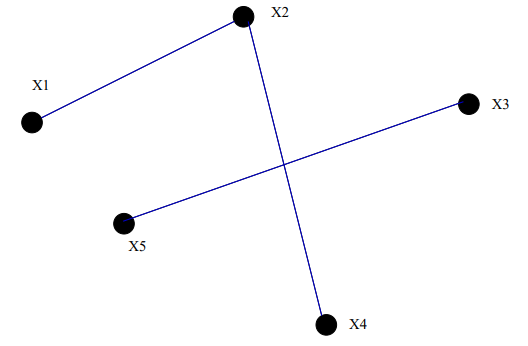
\includegraphics[width=.6\linewidth]{pasted1}
		\captionof{figure}{Time Varying}
		\label{fig:test2}
	\end{minipage}


Now, let us consider if we assumed that both are stationary processes, and we fit an $AR(1)$. If we consider the residuals for the fitted models, we see that the residuals from the time-varying $AR(1)$ model show trends (particularly for $t< 128$) suggesting the model is a poor fit.


	\begin{minipage}{.5\textwidth}
		\centering
		\includegraphics[width=\linewidth]{diag1}
		\captionof{figure}{Stationary}
		\label{fig:test1}
	\end{minipage}%
	\begin{minipage}{.5\textwidth}
		\centering
		\includegraphics[width=1\linewidth]{diag2}
		\captionof{figure}{Time Varying}
		\label{fig:test2}
	\end{minipage}

Now, we estimate the localized autocovariance using a wavelet filter for both realizations. We then plot the localized autocorrelation curves at lags 1,2, and 3 and compare them to the theoretical values we would expect from the fitted models. Clearly, for the time-varying models these observed and theoretical values are vastly different.

	\begin{minipage}{.5\textwidth}
		\centering
		\includegraphics[width=.5\linewidth]{auto1}
		\captionof{figure}{Stationary}
		\label{fig:test1}
	\end{minipage}%
	\begin{minipage}{.5\textwidth}
		\centering
		\includegraphics[width=.5\linewidth]{auto2}
		\captionof{figure}{Time Varying}
		\label{fig:test2}
	\end{minipage}

\section{Discussion and Future Works}

A more general theory can be built using Banach space theory by extending
the idea of using stationary derivative processes approximating locally
stationary process, the benefit is unification of the ergodicity behaviors
(mainly consistency and central limit theorems) as mentioned. The
cost is obvious that very limited possibilities of nonlinearity they
can handle with certain complexity of the processes \cite{Dahlhaus-Richter-Wu}.
Personally I think the work in that direction is pretty much exhausted
although some innovations can be done by relaxation to locally convex
processes. 
\begin{thebibliography}{10}
\bibitem{Brockwell=00003D000026Davis}Brockwell, Peter J., and Richard
A. Davis. Time series: theory and methods. Springer Science \& Business
Media, 2013.

\bibitem{Dahlhaus}Dahlhaus, Rainer. \textquotedbl{}Locally stationary
processes.\textquotedbl{} Handbook of statistics. Vol. 30. Elsevier,
2012. 351-413.

\bibitem{Dahlhaus_96} Dahlhaus, Rainer. \textquotedbl{}Maximum Likelihood
Estimation and Model Selection for Local Stationary Processes. \textquotedbl{}
Nonparametric Statistics. 6 (1996): 171-191.

\bibitem{Dahlhaus_97} Dahlhaus, Rainer. \textquotedbl{}Fitting time
series models to nonstationary processes.\textquotedbl{} The annals
of Statistics 25.1 (1997): 1-37.

\bibitem{Dahlhaus_00} Dahlhaus, Rainer. \textquotedbl{}A Likelihood
Approximation for Locally Stationary Processes. \textquotedbl{} The
annals of statistics. 38.6 (2000): 1762-1794.

\bibitem{Nason et.al}Nason, Guy P., Rainer Von Sachs, and Gerald
Kroisandt. \textquotedbl{}Wavelet processes and adaptive estimation
of the evolutionary wavelet spectrum.\textquotedbl{} Journal of the
Royal Statistical Society: Series B (Statistical Methodology) 62.2
(2000): 271-292.

\bibitem{Cardinali=00003D000026Nason}Cardinali, Alessandro, and Guy
P. Nason. \textquotedbl{}Costationarity of locally stationary time
series.\textquotedbl{} Journal of Time Series Econometrics 2.2 (2010).

\bibitem{Paciorek}Paciorek, Christopher Joseph. Nonstationary Gaussian
processes for regression and spatial modeling Diss. PhD thesis, Carnegie
Mellon University, Pittsburgh, Pennsylvania, 2003.

\bibitem{Ledoux=00003D000026Talagrand}Ledoux, Michel, and Michel
Talagrand. Probability in Banach Spaces: isoperimetry and processes.
Springer Science \& Business Media, 2013.

\bibitem{Dahlhaus-Richter-Wu}\textbackslash{}Dahlhaus, Rainer, Stefan
Richter, and Wei Biao Wu. \textquotedbl{}Towards a general theory
for non-linear locally stationary processes.\textquotedbl{} arXiv
preprint arXiv:1704.02860 (2017). 
\end{thebibliography}

\end{document}
